%% BEGIN INTRODUCTION %%

\chapter{Introduction}
While the field of soluble protein folding has progressed tremendously in the past few decades, membrane protein folding is still in its infancy. \citep{bowie2005, hong2014} The difficulty working with membrane proteins experimentally and the lack of available protein structures in the past limited the amount of studies on the folding of membrane proteins. However, we have seen numerous advances in technology and insights into folding of membrane proteins in the past decade. With more better spatio-temporal resoultion of atomic force microscopy (AFM), we can monitor folding and unfolding of a single turn of a helix in bacteriorhodopsin \citep{yu2017}. With steric-trapping methods, $\Delta$G$^{\circ}_{U}$ of GlpG can be measured in near native environment without the introduction of denaturants. \citep{guo2016} With optical tweezers, GlpG can reversibly fold in a bicelle environment. \citep{min2015} This thesis attempts to further advance the field of membrane protein folding by understanding the folding of potassium channels, an oligomeric membrane protein.

\section{Membrane protein folding}
Membrane proteins are the cell's gateway to its environment. Using a variety of membrane proteins, a cell transmits information, receives nutrients, shapes itself and responds to outside signals. Membrane proteins reside in lipid membranes, and they constitute more than 30\% of the entire proteome. Despite its functional importance and its abundance, our understanding of biochemical and biophysical properties of membrane proteins are still immature because of the difficulties working with membrane proteins experimentally. Membrane proteins easily aggregate because of its high hydrophobicity, and without the correct membrane mimetics, the protein structures can be easily disturbed.

\subsection{$\alpha$-helical versus $\beta$-barrel membrane protein folding}
Generally speaking, membrane proteins can be sub-divided into 2 classes (\textbf{Fig. \ref{fig:intro_f1}}): $\alpha$-helical and $\beta$-barrel membrane proteins. $\alpha$-helical membrane proteins are mainly found in the plasma membrane of eukaryotes, the inner membranes of bacterial cells, and sometimes in the outer membranes of bacteria. They constitute between 20 - 25\% of all open reading frames. On the other hand, $\beta$-barrel membrane proteins are mostly found in the outer membranes of bacteria, mitochondria and chloroplasts, and they constitute only a few percent of all open reading frames. The folding processes for $\alpha$-helical and $\beta$-barrel membrane proteins are very different comprising different sets of chaperones and mechanisms.

\begin{figure}[!ht]
\begin{center}
	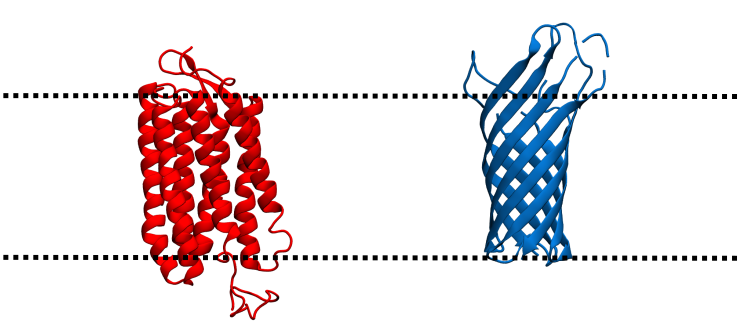
\includegraphics[width=\textwidth]{figures/introduction/Fig1/fig1.pdf}
\end{center}
	\caption{\textbf{$\alpha$-helical versus $\beta$-barrel membrane protein.} Two representative structures of $\alpha$-helical and $\beta$-barrel membrane proteins are shown. Structure of bacteriorhodopsin (PDB ID: 1X0S) monomer is on the left in red, and OmpA (PDB ID: 1BXW) is shown on the right in blue. Theoretical membrane boundaries are drawn in dashed black lines.}
	\label{fig:intro_f1}
\end{figure}

Individual $\alpha$-helices can be stable in the membrane as long as sidechains are hydrophobic enough; however, $\beta$-strands alone are not stable in the membrane because of exposed unsatisfied hydrogen donors and acceptors from the peptide backbone. Due to this basic difference in secondary structure, the mechanism for folding of $\alpha$-helical and $\beta$-barrel membrane proteins are drastically different. $\beta$-barrel membrane proteins insert and fold concurrently whereas $\alpha$-helical membrane proteins will insert one helix at a time and the helices rearrange to fold within the bilayer. In addition, $\beta$-barrel membrane proteins have been shown to fold reversibly from solution containing traditional denaturants such as urea and guanadine hydrochloride (GdnHCl) into lipids. \cite{moon2011, moon2011pnas, moon2013, pocanschi2006, sanchez2008, huysmans2010, hong2004} Because $\beta$-barrel membrane proteins can be monomeric and soluble in traditional denaturants, several proteins' (e.g. OmpA, OmpLA, OmpW, PagP) folding thermodynamics have been measured. \cite{sanchez2008, moon2011, moon2011pnas, moon2013} In which, they found that $\beta$-barrel membrane proteins fold cooperatively by forming $\beta$ sheets at the lipid-water interface and insert simultaneously. 

On the other hand, $\alpha$-helical membrane proteins are highly resistant to urea and GdnHCl, largely due to its hydrophobicity. For folding studies of $\alpha$-helical membrane proteins, the denaturant of choice is sodium dodecyl sulfate (SDS). With SDS, unfolded state of $\alpha$-helical membrane proteins still retain majority of its helicity. \cite{chill2007, booth1995, curnow2007, paslawski2015} Because the SDS-unfolded state still retains a lot of helicity, SDS folding studies mimic \textit{in vivo} folding within the membrane, where the association of helices is the primary driving force for folding. 

The difference in folding mechanism is also reflected in how chaperones help these two classes of proteins fold. For $\beta$-barrel membrane proteins, BAM complexes have been shown to help them insert and fold by thinning the lipid bilayer thickness hence lowering the energy barrier to insert and fold. \cite{gessmann2014, plummer2016} On the other hand, for $\alpha$-helical membrane proteins, ribosomes dock onto the SEC translocons and single helices are synthesized and inserted into the membrane one at a time as shown in Figure \ref{fig:intro_f2}. Many advances have been made in the field of $\beta$-barrel membrane proteins and there are excellent reviews available. Here in this thesis, the focus will be on the folding of $\alpha$-helical membrane proteins.

\subsection{The two stage model and beyond}
In 1990, the two stage model was proposed to provide a general framework for folding of $\alpha$-helical membrane proteins fold as shown in Figure \ref{fig:intro_f2}. The model was proposed based on refolding studies of bacteriorhodopsin, where the Popot and Engelman showed that bacteriorhodopsin can still re-assemble after being cut in different loops. Based on these results, Popot and Engelman proposed that $\alpha$-helical membrane proteins must first insert into the membrane, then helices associate laterally to fold into its native state.

\begin{figure}[!ht]
\begin{center}
	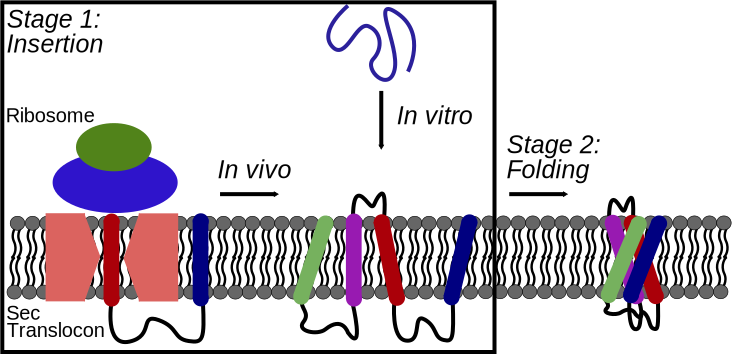
\includegraphics[width=\textwidth]{figures/introduction/Fig2/two_stage.pdf}
\end{center}
	\caption{\textbf{Two stage folding process for membrane protein folding.} The first stage of the membrane protein folding process is insertion, where single helices are synthesized and inserted into the bilayer one at a time. As noted above, the insertion process is different for \textit{in vivo} and \textit{in vitro}. However, upon insertion of helices into the membrane, folding within the membrane is thought to process via the same pathway.}
	\label{fig:intro_f2}
\end{figure}

In the two stage model, the first stage of membrane protein folding is called insertion, where the protein gets inserted into the membrane with its native-like secondary structures. This process is very different for \textit{in vivo} and \textit{in vitro}. \textit{In vivo}, single helices are secreted from the ribosome directly into SEC translocons, then the helices are transferred from the translocon into the lipid bilayer. However, \textit{in vitro}, the unfolded peptide transfers directly from solution into the lipid bilayer. For many biochemical and biophysical studies using \textit{in vitro} systems, the folding process is hard to study because during the \textit{in vitro} insertion process, many membrane proteins can misfold and aggregate.

For \textit{in vivo} insertion, the exact mechanism on how a single helix transfers from inside the SEC translocon into the bilayer is not well understood yet, but the transfer is thought to happen via a lateral gate that opens in the translocon. A more recent model suggests that helices move between inside of the translocon, lipid-water interface, and the hydrophobic core of the membrane. Regardless, the insertion process is largely determined by the hydrophobicity of the peptide segment. Using amino acid hydrophobicity scales and sliding window averages, transmembrane segments can be predicted well. However, for some systems like LacY, the overall topologies can be flipped by changing the lipid compositions \textit{in vivo} and \textit{in vitro}. \cite{bogdanov2010, vitrac2013, vitrac2015}

After successful insertion of helices into the membrane, the helices begin to undergo lateral association, which is described as folding within the membrane. This process is determined by many different forces including protein-protein and protein-lipid interactions, and lateral pressure of the membrane. The major driving force for helix-helix interactions are still not clear. There are many competing forces which can drive helix-helix association hydrogen bonds, van der Waals interaction, polar side-chain burial, and salt bridges.


\begin{figure}[!ht]
\begin{center}
	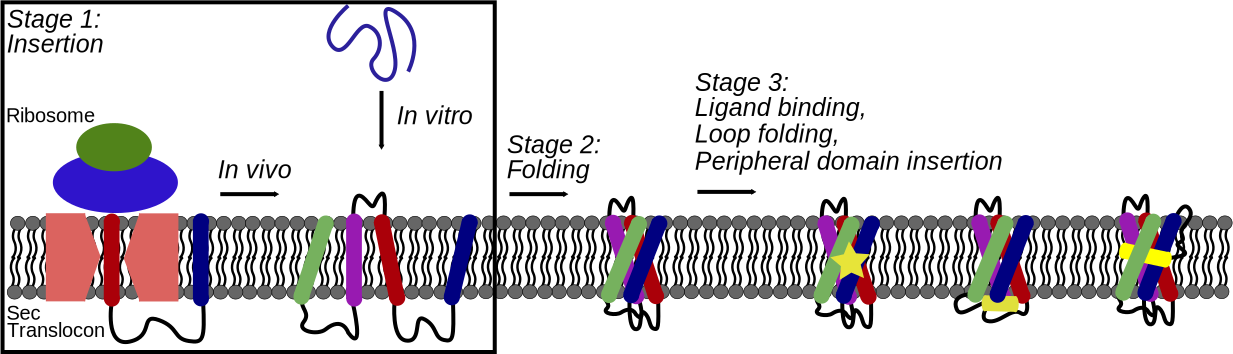
\includegraphics[width=\textwidth]{figures/introduction/Fig3/three_stage.pdf}
\end{center}
	\caption{\textbf{Three stage model for membrane protein folding.} The first two stages are identical to the two stage model as shown in Figure \ref{fig:intro_f2}. The third stage can be a variety of events, such as ligand binding, folding of the loops and/or peripheral domain insertion.}
	\label{fig:intro_f3}
\end{figure}

In the two stage model, insertion and lateral association of helices would complete the folding of membrane proteins. However, many membrane proteins require more intricate folding even after association of helices have completed. Therefore, a more detailed three stage model was proposed as shown in Figure \ref{fig:intro_f3}. \cite{engelman2003} This model proposes that further folding happens after lateral helix association, which can include binding of a ligand, folding of loop regions and insertion of peripheral domains into the bilayer. In case of multimeric membrane proteins like many ion channels, another step is required where monomeric subunits must associate to form native channels, which will be discussed further in the following sections. 

\section{Potassium channels}
\subsection{Potassium channel function and diseases}
Potassium channels are found in all kingdoms of life. From bacteria to humans, the basic function of potassium channels is to selectively regulate the flow of K$^{+}$ ions across cell membranes. While the basic functions are identical across organisms, potassium channels have many different uses in different organisms. In prokaryotes, potassium channels are responsible for cell growth and survival. For biofilms, the community of microorganisms use potassium channels to communicate with each other to coordinate their feeding cycles. \cite{prindle2015,liu2015} 

In humans, potassium channels are used to drive muscle contraction and neuronal signaling. Because of their significant role in human physiology, the proper functioning of potassium channels are critical to human health. There are over 50 known genes encoded for potassium channels in humans, and mutations to any of these potassium channels presumably results in a disease. \cite{shieh2000} Some examples include long-QT syndromes, \textit{Weaver} syndrome, familial convulsions, hearing and vestibular diseases, Bartter's syndrome, and familial persistent hyperinsulinemic hypoglycemia of infancy.

Two of the most well-known diseases related to potassium channel mutations are long-QT (LQT) syndromes and \textit{Weaver} syndromes. LQT syndromes are cardiac diseases that affect the rhythm of the heart beat. This genetically inherited disease can cause heart to suddenly beat faster and more chaotically. With prolonged chaotic beating of the heart, this disease can cause sudden death in people with LQT syndromes. Mutations in KCNQ1 and hERG genes can cause a variety of LQT syndromes. \cite{shieh2000} Studies of some of the more common mutations in these genes showed that assembly and proper trafficking of these potassium channels to plasma membrane of the cell is diminished in these mutants, which causes the heart to beat erratically. 

Whereas LQT syndromes affect the function of the heart, \textit{Weaver} syndromes affect the function of neurons with similar symptoms as Parkinson's diseases, resulting in severe tremors and loss of control of motor functions. In some cases, symptoms can also include male infertility, and sporadic seizures. The \textit{Weaver} was mapped to a single mutation (G156S) in the pore region of Kir3.2 potassium channel. This mutation renders Kir3.2 potassium channel to be non-selective, letting sodium ions through as well as potassium ions.

The importance of potassium ion channels in physiology is indisputable. Many functional studies utilizing electrophysiology techniques exist for potassium ion channels, and there are more potassium ion channel structures being generated through advances in X-ray crystallography and Cryogenic electron microscopy studies. However, the folding process of potassium channel is largely uncharacterized. Understanding the folding of potassium ion channels will be important as LQT and \textit{Weaver} syndromes are all caused by folding defects of potassium ion channels.

\subsection{Potassium channel structure}

\begin{figure}[!ht]
\begin{center}
	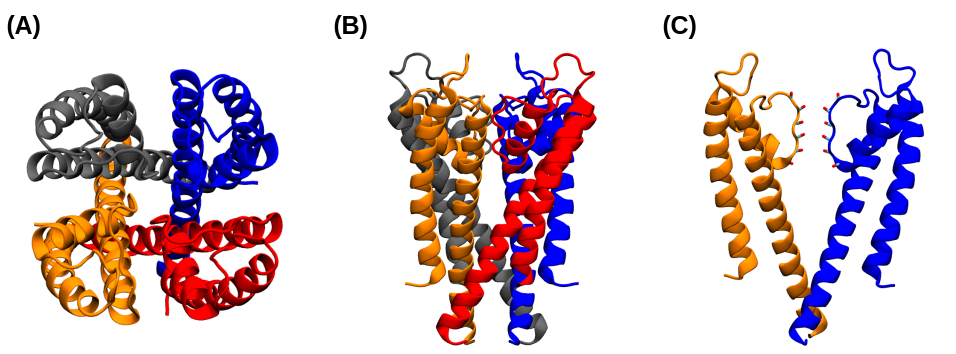
\includegraphics[width=\textwidth]{figures/introduction/Fig4/Fig4.pdf}
\end{center}
	\caption{\textbf{Structure of KcsA (PDB ID: 1R3J) shown from different angles}. \textbf{(A)} KcsA shown from the extracellular side of the membrane. \textbf{(B)} KcsA shown from the side. \textbf{(C)} KcsA viewed from the side with 2 monomers removed for better visualization of the selectivity filter. The oxygen atoms lining the selectivity region is rendered in Licoriche mode and the protein structures are rendered in New Cartoon mode in VMD. Each monomer of KcsA is colored in grey, blue, orange and red.}
	\label{fig:intro_f4}
\end{figure}

The first structure of potassium channel \ref{fig:intro_f4} was solved in 1998 by Roderick MacKinnon's lab, which he was awarded the Nobel Prize in Chemistry for in 2003. The structure showed that the pore is formed by the juxtaposition of 4 subunits along the symmetry axis. The pore is lined with oxygen atoms from the backbone of the selectivity filter residues (\textbf{Fig. \ref{fig:intro_f4}C}). Thes oxygen atoms provide binding 4 sites for K+ ions as they pass through the pore. The pore selectively allows K$^{+}$ ions to flow through excluding other ions including Na$^{+}$, which has similar metallic structure as K$^{+}$ ions. Because of this important function of the potassium channel pore, the pore region is highly conserved amongst its family members. In particular, \textbf{TVGYG} sequence in the selectivity filter region is highly conserved. 

In terms of potassium channel folding, several biophysical properties of K+ channels are relevant to their dynamics. The ion-conducting pore of K+ channels, formed by the re-entrant segment located between the two hydrophobic TM helices, is lined with polar and charged residues. If the helices retained the same structure and orientation as they do in the tetramer, the polar residues along with the non-hydrogen-bonded backbone atoms would be exposed to lipids in its monomeric form. As these interactions are energetically unfavorable, the dominant conformation of individual monomers prior to tetramerization is unclear. Previous thiol-labeling experiments have shown that for Kv1.3, the monomers maintain the helical structure of the re-entrant p-helix in a native-like orientation.20-21 Likewise, MD simulations indicated that the monomers’ native conformation was stable on a timescale of ~1 s.21 These results demonstrated that the p-helix remains helical and lies at the water-lipid interface, however, the relative orientation of the 2 TM helices and the p-helix is not known.
 
\section{Potassium channel folding}
\subsection{Folding of KcsA}
One of the first evidence that KcsA can be refolded from a completely unfolded form came from Valiyaveetil et al. \citep{valiyaveetil2002semi} The study showed that the N-terminal fragment corresponding to residues 1 -- 73 of KcsA can be recombinantly expressed in \textit{E. coli}, and a synthetic C-terminal fragment corresponding to residues 74 -- 125 can be chemically ligated. Once, the two fragments are ligated, KcsA can be refolded into tetramers for dilution of the monomers into solutions containing liposomes. While this study showed that KcsA can be refold into tetramers, the paper did not explore kinetics or thermodynamics of refolding in detail. Regardless, this study was the first to show that KcsA can be chemically synthesized and refolded from an unknown unfolded state.

In the following years, several papers detailing unfolding and reversible folding KcsA using 2,2,2-trifluoroethanol (TFE) were published. \citep{molina2004, barrera2005, barrera2008} The studies showed that at lower TFE concentrations, Trp fluorescence can be monitored to measure folding and unfolding of KcsA reversibly. However, at higher TFE concentrations, KcsA does not refold. While this study first suggested that TFE might be a good reagent to monitor reversible refolding of KcsA, the study overall did not provide much insight into the kinetics or thermodynamics of the folding process. In addition, TFE is known to promote helicity in proteins, so the nature of TFE-induced unfolded state of KcsA is not clear. However, through the TFE studies, the tetramer was proposed to unfold first via the pore helix region and then the separation of all subunits at high TFE concentration leads the proteins to irreversibly aggregate.

The TFE studies gave insights into the thermodynamics of KcsA folding; however, currently, there are no known kinetics studies of the folding of potassium channels. In addition, we do not have a good grasp of what's happening at the atomic and molecular level in KcsA folding.

\subsection{Folding of voltage-sensing potassium (Kv) channels}
The first folding studies of Shaker-type voltage-gated potassium channel studied the effect of deleting the tetramerization (T1) domain on the kinetics of tetramerization process. \cite{zerangue2000} The study showed that while the mutant without the T1 domain can still function as a tetramer, channel formation was dramatically reduced. Upon introducing GCN1, a parallel helical tetramer, into T1 region, channel formation was rescued. Based on this result, the T1 domain was suggested to help channels form by first forming tetramers and letting the pore domain fold in sequence. This result provided a glimpse of how potassium channels fold. They first partition into oligomers by the T1 domains associating with each other, allowing the transmembrane domains to fold subsequently. 

The first \textit{in vitro} folding of Kv channels was done with K$_{v}$AP, which is a voltage-sensitive potassium channel found in archeabacterium, \textit{Aeropyrum Pernix}. \cite{devaraneni2011} Interestingly, the study showed that K$_{v}$AP insert quickly into the bilayer at room temperature or at 80 $^{\circ}$C; however, folding into tetramers is much more efficient at 80 $^{\circ}$ than it is at room temperature. This is the first study to demonstrate a refolding assay using SDS-PAGE and quenching of the refolding reaction with SDS, and also the first study to show almost complete refolding of multi-domain membrane protein in a bilayer.

While the above studies showed the folding of Kv channels at more global level, more studies came out that began to elucidate the structure of potassium channel monomers in bilayer at atomic level. Using a novel mass-tagging and molecular tape measure, Gajewski et al. showed that the Kv1.3 monomers can immediately begin to form secondary structures as they exist the ribosome-translocon complex. In addition, with 650 ns of simulations and van der Waals calculations, the monomeric structure of Kv1.3 pore domain was thought to be stable in the structure found in native-like tetramers.

Using similar thiol-labeling methods, the structure of pore helix was probed further. By scanning the pore helix region with cysteines and measuring the rate of pegylation along all the helical sites, the pore helix was found to retain its native-like secondary structures. The rate of pegylation varied in a helical pattern suggesting that one side of the helix is more buried than the other. Then, using a fixed cysteine mutation site and introducing mutations at different site along the p-helix, some of the key residues that change the orientation of the pore helix was found. However, overall, Delaney et al. was the first to show experimentally that the pore helix retains its native-like helical secondary structure.

\section{Aims and significance}
\subsection{Understanding the dynamics of potassium channel monomers}
Through molecular dynamics (MD) simulations and nuclear magnetic resonance (NMR) spectroscopy, we first study the dynamics of potassium channel monomers in lipid-like environment. From previous studies, the structure of potassium channel monomers at the molecular level is not well characterized. Delaney et al. demonstrated that the monomers will retain its native-like secondary structures, but whether the tertiary structures are retained is not established. The goal of this section is to characterize the dynamics of the potassium channel pore domain monomers at the atomic level.

\subsection{Biochemical prepartion of WT KcsA and more native-like mutant monomers}
KcsA is an extremely stable membrane protein in its native tetrameric form. In order to prepare stable monomer samples, we adopt several different biochemical prepartion protocols to prepare monomeric potassium channels. In addition, we designed a KcsA mutant that retains its native-like structure more than the WT KcsA monomer does. The protocols and results verifying the biochemical prepartion of WT and mutant KcsA monomer is discussed.

\subsection{Connecting the dynamics of potassium channel monomers to the assembly process}
With the use of gel-based refolding assay and FRET, we investigate the folding kinetics of WT KcsA and the more native-like mutant with a disulfide-bridge (CC) mutant. Concentration dependent study of the refolding kinetics show that the tetramerization process does not have a concentration dependence despite the native state of the protein being a tetramer. This suggested that the rate-limiting step is unimolecular and led us to hypothesize that the proteins might form an early molten globule structure prior to folding into native tetramers. We verify the 

\subsection{Significance}
Here in this thesis, we connect the dynamics of potassium channel monomers to the kinetics of tetramerization. Far from being a simple association of pre-formed monomers, they initially exist as a heterogeneous ensemble in a protein-rich phase in the membrane, which may be a general phenomenon. Tetramerization kinetics indicate that the rate-limiting step is unimolecular despite the native state being a tetramer. Folding can occur along fast or slow (misfolded) pathways that can be modulated with mutants that trap monomers in a native-like state. In spite of its name, the C-terminal “tetramerization” domain in KcsA does not enhance tetramerization, suggesting it plays another role in channel function.

%%\newpage
%%The aims of my studies are:
%%\begin{itemize}
%%\item Determine the structural state of potassium channel monomers in lipid bilayers
%%\item Determine the folding pathway of potassium channels
%%\end{itemize}

%% END INTRODUCTION %%

